\documentclass[main.tex]{subfiles}


\begin{document}


\subsection{Frameshift stimulating elements of multiple coronaviruses form long-range RNA--RNA interactions}

We hypothesized that similar long-range interactions could exist in other coronaviruses -- particularly other SARS-related viruses.
To test this hypothesis, we performed SEARCH-MaP with FSE-targeted ASOs on 1,799 nt segments from eight selected coronaviruses.


\subsubsection{Computational and experimental screening identifies eight coronaviruses with potential long-range interactions}

As of December 2021, the NCBI Reference Sequence Database~\cite{OLeary2016} contained sixty-two complete genomes of coronaviruses.
To focus on those likely to have long-range interactions involving the FSE, we predicted the likelihood that each base in a 2,000 nt section surrounding the FSE would pair with a base in the FSE (SFIG).
Based on these predicted interactions, we selected ten coronaviruses (including SARS-CoV-2) for further study -- at least one from each genus (SFIG).
Within the genus \textit{Betacoronavirus}, we included all three of the SARS-related viruses -- SARS coronaviruses 1 (\verb|NC_004718.3|) and 2 (\verb|NC_045512.2|) and bat coronavirus BM48-31 (\verb|NC_014470.1|) -- because they clustered into their own structural outgroup, distinct from all other coronaviruses.
The other three strains of \textit{Betacoronavirus} that we selected were MERS coronavirus (\verb|NC_019843.3|) with a predicted interaction at positions 510-530; and human coronavirus OC43 (\verb|NC_006213.1|) and murine hepatitis virus strain A59 (\verb|NC_048217.1|), both with a predicted upstream interaction at positions 10-20.
We selected two strains of \textit{Alphacoronavirus}: transmissible gastroenteritis virus (\verb|NC_038861.1|) and bat coronavirus 1A (\verb|NC_010437.1|), predicted to have interactions at positions 440-460 and 350-360, respectively.
Avian infectious bronchitis virus strain Beaudette (\verb|NC_001451.1|) -- a strain of \textit{Gammacoronavirus} -- was predicted to have a strong interaction at positions 330-350, while common moorhen coronavirus HKU21 (\verb|NC_016996.1|) was the species of \textit{Deltacoronavirus} with the most promising FSE interactions.

We reasoned that if an FSE does interact with a distant RNA element, then removing that element by truncating the RNA would break the interaction, causing a structural change in the FSE that could be detected though chemical probing.
For each of the ten coronaviruses that passed the computational screen, we \textit{in vitro} transcribed and performed DMS-MaPseq~\cite{Zubradt2016} on both a 239 nt segment comprising the FSE and minimal flanking sequences and a 1.8 kb segment encompassing the FSE and all sites with which it was predicted to interact.
All coronaviruses except for human coronavirus OC43 and MERS coronavirus showed differences in their DMS reactivity profiles between the 239 nt and 1.8 kb segments (SFIG), suggesting long-range interactions between the FSE and another element within the 1.8 kb segment.


\subsubsection{SEARCH-MaP reveals long-range interactions involving the FSE in five coronaviruses}

To determine whether the FSE interacts with another RNA element -- and if so, which -- in each coronavirus, we performed SEARCH-MaP on the 1.8 kb RNA segment using ASOs targeting the bases that changed the most between the 239 nt and 1.8 kb segments.
Using SEISMIC-RNA, we computed the mutational profiles with and without ASOs and calculated the Spearman correlation coefficient (SCC) between them via a sliding window (Figure \ref{covs}).
In every coronavirus, the ASO target site (light green) showed a large dip in SCC, confirming that the ASOs bound and altered the structure.

The long-range interaction in SARS-CoV-2 was suggested to comprise three stems~\cite{Ziv2020}.
SEARCH-MaP found two (dips in SCC around positions 1,500 and 1,615); the third stem (around position 1,375) may have been missed because it is not only the shortest (15 nt) but also has just one unpaired base on each side.
Similar long-range interactions appeared in the other SARS-related viruses: SARS-CoV-1 and bat coronavirus BM48-31.
Like SARS-CoV-2, both had a dip in SCC near position 1,500 and another dip downstream, between positions 1,575 and 1,675. 
The SCC also dipped around position 1,375 for SARS-CoV-1, matching the location of the missed stem in SARS-CoV-2.
Therefore, this three-stemmed long-range interaction involving the FSE appears to be conserved among three strains of SARS-related viruses, suggesting it is functional.

Examining the other species, we found prominent dips in SCC below 0.9 further than 200 nt from the ASO target site in all except common moorhen coronavirus.
We modeled potential structures for these long-range interactions using the Fold program from RNAstructure~\cite{Mathews2004a} with the no-ASO mutational profiles as DMS constraints~\cite{Cordero2012}.
The computationally predicted structures for murine hepatitis virus and transmissible gastroenteritis virus were consistent with the SEARCH-MaP data (Figure \ref{covs}).
We subsequently focused on transmissible gastroenteritis virus because its long-range interaction lay downstream of the FSE, as in the SARS-related viruses.


\begin{figure}[ht]
	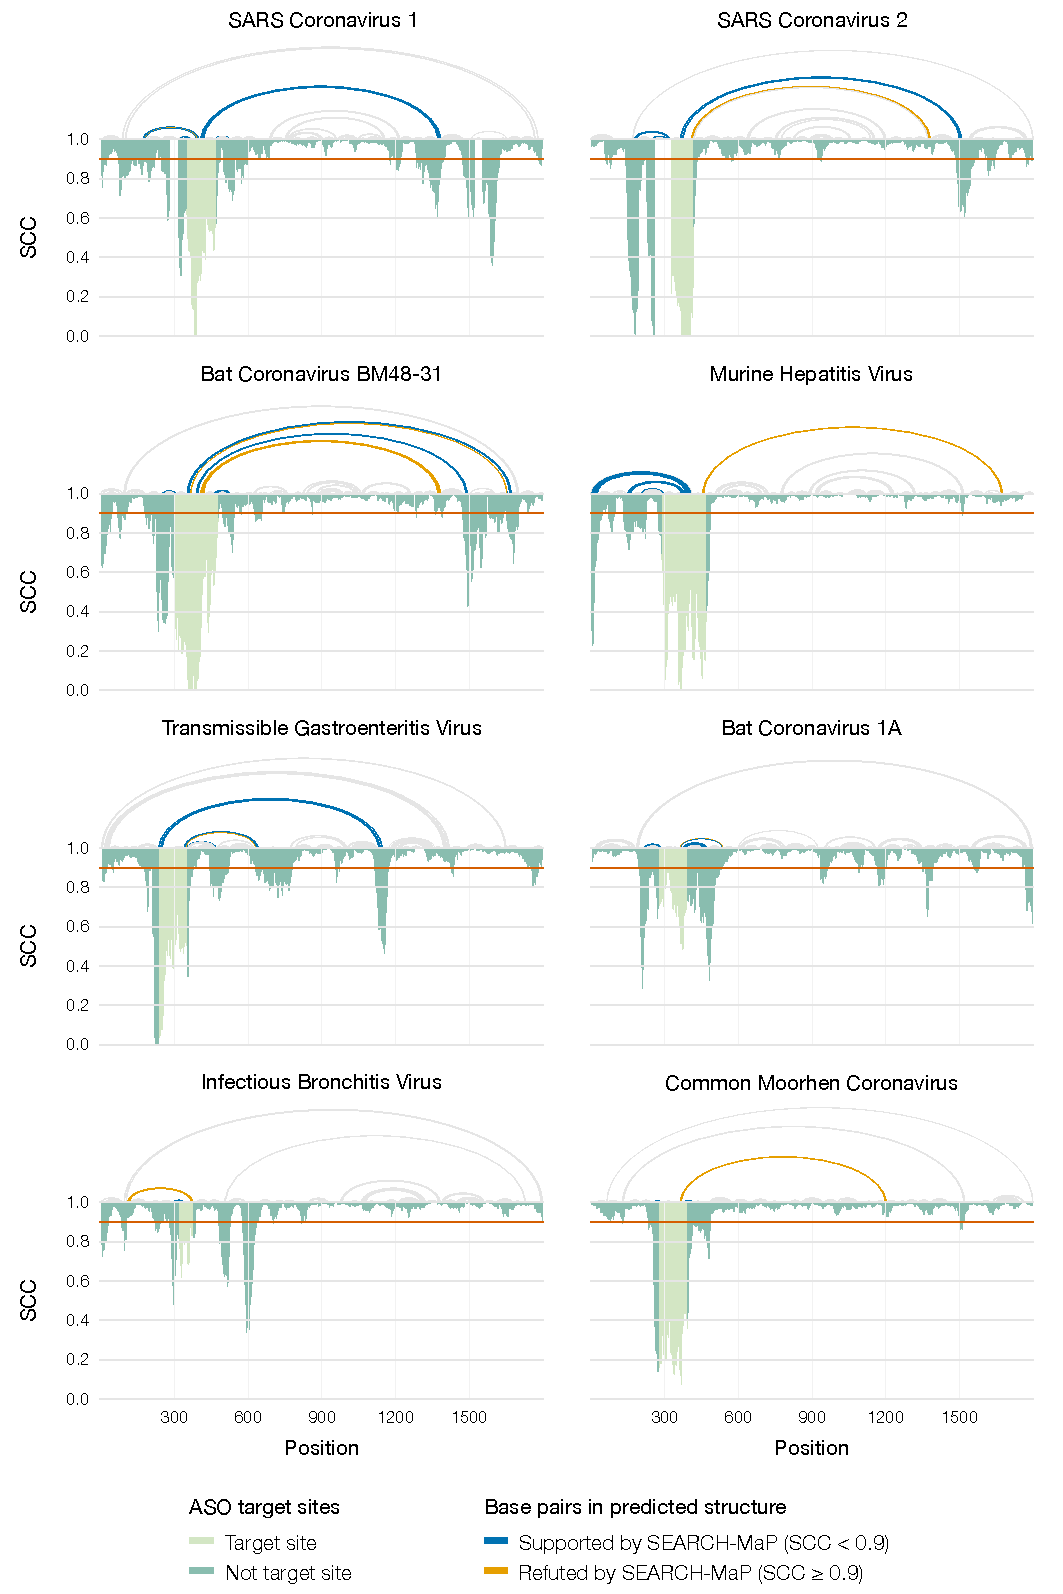
\includegraphics[height=0.95\textheight]{../MainFigures/covs/covs.pdf}
	\caption{}
	\label{covs}
\end{figure}


\end{document}
